\documentclass[dvipdfmx, a4paper, 11pt]{jsarticle}

% --- 日本語環境用設定 ---
\usepackage[top=25truemm,bottom=25truemm,left=25truemm,right=25truemm]{geometry}

% --- 追加パッケージ ---
\usepackage[dvipdfmx]{graphicx} % 画像読み込み用
\usepackage{booktabs}           % 表の罫線を美しくする
\usepackage{url}                % URLの表示
\usepackage{float}              % 図表の位置固定 [H] 用
\usepackage{amsmath}            % 数式

\graphicspath{{../results/}}

% --- 箇条書き設定（パッケージを使わない方法に変更）---
\renewcommand{\labelitemi}{--}

% --- タイトル情報 ---
\title{分析2 小レポート：\\YouTubeコメントのLLM構造化コーディング\\ \large{―打ち切り時点の集計（$N=14{,}501$，目標18,000件中約84\%）―}}
\author{明治大学 政治経済学部 杉本ゼミ\\ 牧野 杏珠}
\date{\today}

\begin{document}

\maketitle

\begin{abstract}
本レポートは，卒業論文第4部・分析2（YouTubeコメントのLLM構造化コーディング）
の結果を要約する内部メモである。財務省デモ・参政党・不法移民の3トピック
についてYouTube日本語コメント計38{,}214件を収集し，トピックごと最大
6{,}000件（合計18{,}000件）の層化サンプルに対し，ローカルLLM（Ollama,
qwen2.5:7b-instruct）による6変数の構造化コーディングを実施した。本レポート
は，\texttt{src/analyze\_coding.py}を最後に実行した時点（コーディング済み
15{,}187件，parse\_error 0件，スパム除外後$N=14{,}501$，目標18{,}000件の
約84\%）の結果を報告する。コーディング処理自体はバックグラウンドで継続中
であり，本レポート脱稿後にさらに件数が増える可能性があるが，
\textbf{本レポートおよび卒論本文はこの84\%時点の数値を最終的な分析対象
として採用する}。結果は，\texttt{people\_vs\_elite}（人民対エリート）が
財務省デモで28.1\%と突出し，\texttt{economic\_resentment}（経済的怨恨）は
いずれのトピックでも1--4\%と低く，\texttt{theft\_of\_enjoyment}（享楽の
盗取）は不法移民トピックでのみ6.8\%と突出するという，トピックごとに大きく
異なるパターンを示している。この傾向は，コーディング完了率31\%・41\%・
84\%という3つの時点を通じて安定して観察されている。ただし人手検証
（Cohenの$\kappa$）の結果，\texttt{economic\_resentment}と
\texttt{theft\_of\_enjoyment}の測定信頼性はほぼゼロであり，この2変数に
基づく結論は暫定的な知見にとどめる必要がある。
\end{abstract}

\section{分析の目的と位置づけ}
分析1（\texttt{analysis/survey\_regression/}）は，既存の大規模社会調査
データを用いてSNS利用と制度への信頼というマクロな量的関係を検証したが，
SNS利用の効果は統計的に非有意であった。分析2は，この非有意性が「SNSが
日本の政治と無関係である」ことを意味するのではなく，SNSの影響が制度への
信頼のような静的な態度指標としては現れにくく，具体的な言説の内容や
トーンのレベルでこそ観察されるのではないか，という仮説を検証するために
設計されている。理論編（第1--3部）で導入した「人民対エリート」
（Mudde \& Rovira Kaltwasser, 2017）・「経済的怨恨」（Ricci, 2020）・
「享楽の盗取」（Kawamura \& Iwabuchi, 2022）といった概念を，YouTube
コメント1件単位の変数へ操作化し，構造化コーディングによって検証する。

\section{データ収集}
収集対象は3トピック：(1) 財務省デモ・財務省解体・減税，(2) 参政党，
(3) 不法移民・外国人問題。複数の検索クエリによる動画検索と著者による
手動選定を組み合わせ，計153本の動画から38{,}214件のコメント
（トップレベル・返信を含む）を収集した（内訳：不法移民16{,}020件，
財務省デモ15{,}050件，参政党7{,}144件）。収集はYouTube Data API v3を
用いて2026年8月11--12日に実施した。

\paragraph{収集順序に由来するバイアス}
コメント取得は投稿時系列（\texttt{order="time"}）ではなく，YouTube API
独自の「関連性」順（\texttt{order="relevance"}，実質的にはエンゲージメント
指標に基づくランキング）で行っている。したがってサンプルは各動画で
\emph{最もエンゲージメントの高い}コメントに事実上限定されており，
感情的・対立的な言説へ体系的に偏っている可能性が高い。この点は
\texttt{people\_vs\_elite}等の出現率を「典型的な水準」ではなく
\emph{上限に近い推定値}として解釈すべき理由になる。

\section{前処理}
コメントID基準の重複除去，URL除去・空白正規化，クレンジング後5文字未満の
極端に短いコメントの除外という3段階の前処理を行った。生コメント
38{,}656件のうち442件（1.1\%）が除外され，38{,}214件が分析対象として
残った。スパム・話題逸脱コメントの判別は前処理段階では行わず，後述の
\texttt{is\_spam\_or\_offtopic}変数（LLMコーディング）に委ねている。

\section{構造化コーディングの手法}

\subsection{モデルと変数}
ローカルLLM（Ollama, qwen2.5:7b-instruct, temperature=0）を用い，
コメント本文を外部クラウドAPIへ送信しないプライバシー配慮と，
モデル・パラメータ固定による再現性を優先した。操作化した6変数は
表\ref{tab:variables}の通りである。

\begin{table}[H]
\centering
\caption{コーディングスキーム（\texttt{config/coding\_scheme.yaml}）}
\label{tab:variables}
\begin{tabular}{lll}
\toprule
変数名 & 型 & 理論的根拠 \\
\midrule
\texttt{people\_vs\_elite} & 真偽値 & Mudde \& Rovira Kaltwasser (2017), pp.5--6 \\
\texttt{economic\_resentment} & 真偽値 & Ricci (2020), pp.viii--ix, p.52 \\
\texttt{theft\_of\_enjoyment} & 真偽値 & Kawamura \& Iwabuchi (2022) \\
\texttt{blame\_target} & カテゴリ（7値） & Fujishiro et al. (2020), p.315 \\
\texttt{emotional\_tone} & カテゴリ（5値） & Bennett \& Livingston (2020) \\
\texttt{is\_spam\_or\_offtopic} & 真偽値 & 分析対象からの除外フラグ \\
\bottomrule
\end{tabular}
\end{table}

\subsection{標本抽出}
全38{,}214件ではなく，トピックごと最大6{,}000件（合計18{,}000件）を
無作為抽出した層化サンプル（乱数シード42，再現可能）を対象にコーディング
している。全件コーディングは実測処理時間（1件あたり約7--25秒，計算機の
負荷状況により変動）から換算すると136時間超を要するため，計算資源の
制約から標本抽出を行い，さらに後述の通り目標件数の途中でコーディングを
打ち切っている。

\section{打ち切り時点についての明記}
\label{sec:cutoff}
コーディング処理は\texttt{comment\_id}単位で既処理分をスキップして
再開できる設計であり，計算機を起動できる時間帯にバックグラウンドで
断続的に実行してきた。表\ref{tab:progress}に主要な時点での進捗を示す。

\begin{table}[H]
\centering
\small
\caption{コーディング進捗のスナップショット}
\label{tab:progress}
\begin{tabular}{p{4.5cm}p{4.5cm}c}
\toprule
時点 & ラベル済み件数 & 割合 \\
\midrule
中間時点1 & 5{,}584件 & 31\% \\
中間時点2 & 7{,}480件（スパム除外後7{,}144件） & 41\% \\
\textbf{本レポートの集計対象} & \textbf{15{,}187件}（スパム除外後14{,}501件） & \textbf{84\%} \\
\bottomrule
\end{tabular}
\end{table}
表中の「本レポートの集計対象」は，最終的に\texttt{analyze\_coding.py}を
実行した時点を指す（割合は目標18{,}000件に対する比率）。

本レポートおよび卒論本文は，この84\%時点（$N=14{,}501$）を
\textbf{最終的な分析対象}として採用する。目標の全件完了を待たずに
打ち切ったという判断自体が，本稿の分析2が抱える最大の限界の一つであり，
以下で報告する出現率・検定結果は，最終的にコーディングされるであろう
18{,}000件全体の値ではなく，この84\%時点のサブサンプルにおける値である
点を明記しておく。コーディング処理自体はバックグラウンドで継続中であり，
本レポート脱稿後にさらに件数が増える可能性があるが，その場合も
\texttt{analyze\_coding.py}を再実行するまでは本レポートの数値が有効な
最新版である。

31\%→41\%→84\%という3つの時点で同一の集計を実施しており，第
\ref{sec:results}節で示す通り，出現率・事前規定基準の適用結果はこれら
3時点を通じて質的に安定している。

\section{結果（$N=14{,}501$時点）}
\label{sec:results}

\subsection{変数の出現率}
\texttt{is\_spam\_or\_offtopic}に該当するコメント（686件）を除いた
14{,}501件について，Wilsonスコア区間（95\%）とともに算出した出現率を
表\ref{tab:prevalence}に示す。

\begin{table}[H]
\centering
\caption{トピック別の変数出現率（95\%Wilsonスコア区間）}
\label{tab:prevalence}
\begin{tabular}{lccc}
\toprule
 & 財務省デモ & 参政党 & 不法移民 \\
\midrule
\texttt{people\_vs\_elite} & \textbf{28.1\%} [26.7, 29.5] & 10.7\% [9.7, 11.7] & 5.6\% [4.9, 6.3] \\
\texttt{economic\_resentment} & 3.6\% [3.1, 4.3] & 0.9\% [0.6, 1.2] & 1.4\% [1.1, 1.8] \\
\texttt{theft\_of\_enjoyment} & 0.8\% [0.6, 1.1] & 0.8\% [0.5, 1.1] & \textbf{6.8\%} [6.1, 7.6] \\
\bottomrule
\end{tabular}
\end{table}

3トピックを併せた全体では，\texttt{people\_vs\_elite}が14.56\%
[13.95, 15.20]（$N=12{,}270$），\texttt{economic\_resentment}が1.98\%
[1.75, 2.24]（$N=12{,}270$），\texttt{theft\_of\_enjoyment}が2.93\%
[2.65, 3.25]（$N=12{,}273$）である。これらの値は，31\%時点（それぞれ
13.6\%，2.2\%，3.4\%）・41\%時点（13.9\%，2.15\%，3.2\%）と比べても
大きく変動しておらず，サンプルサイズの拡大に対して安定している。

\texttt{people\_vs\_elite}は財務省デモで突出して高く，反政府的な動員の
言説的特徴と整合する。\texttt{economic\_resentment}はいずれのトピックでも
低く（1--4\%），Ricciが想定する経済的怨恨がこのサンプルの範囲では言説
として顕在化しにくいことを示唆する。\texttt{theft\_of\_enjoyment}は
不法移民トピックに強く偏在しており，Kawamura \& Iwabuchi (2022)の理論が
本来想定する民族的トピックの範囲内で明確に観察される。

\subsection{blame\_targetの分布：カイ二乗検定}
非難の矛先（\texttt{blame\_target}）の分布はトピック間で統計的に極めて
有意に異なる（$\chi^2(10)=4688.83$，$p<0.000001$，Cramér's $V=0.587$，
大きな効果量）。標準化残差を見ると，財務省デモは\texttt{elites\_general}
（残差$+40.3$）に，参政党は\texttt{specific\_party}（残差$+43.2$）に，
不法移民は\texttt{immigrants}（残差$+40.4$）・\texttt{foreign\_country}
（残差$+24.6$）に，それぞれ強く偏って集中している（図\ref{fig:heatmap}）。
カイ二乗統計量は41\%時点（$\chi^2=2282.14$）よりおよそ2倍に増大している
が，これは標本サイズの増加に伴う機械的な増大であり，関連の実質的な強さを
表すCramér's $V$は0.584→0.587とほぼ変化していない。これはFujishiro et
al. (2020)の「排外主義対リベラル」という単一軸ではなく，トピックごとに
非難の対象そのものが体系的に異なる，より分節化した構造を示唆する。

\begin{figure}[H]
    \centering
    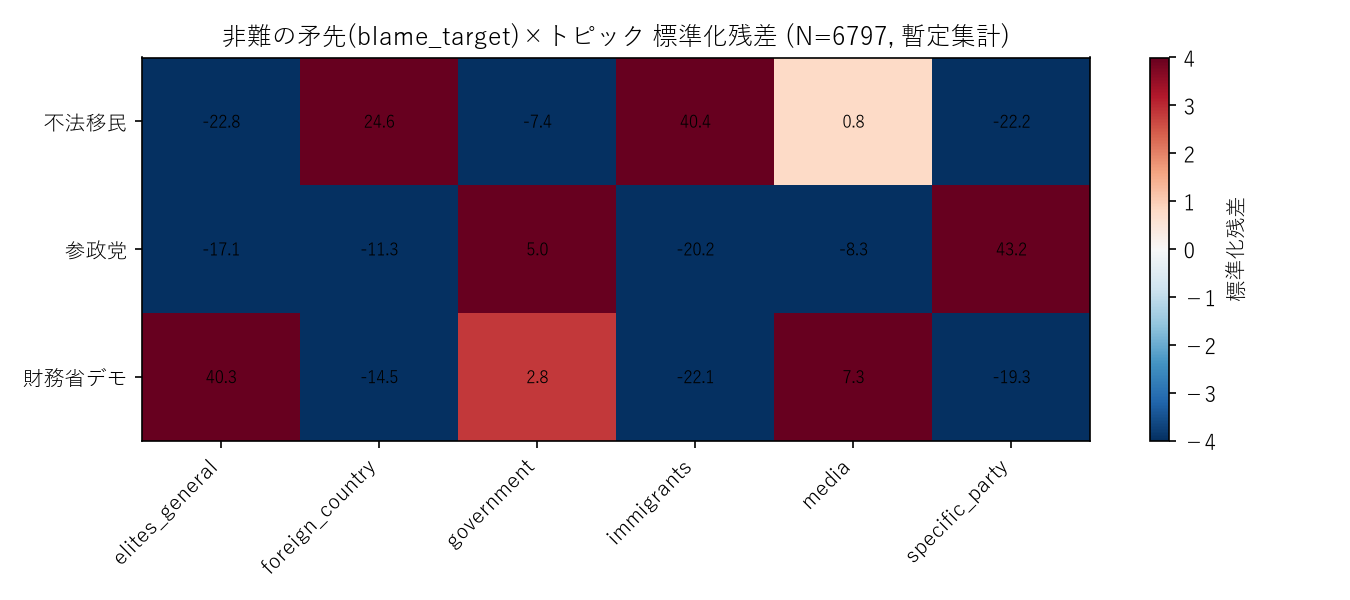
\includegraphics[width=0.85\textwidth]{coding_blame_target_heatmap_14501.png}
    \caption{blame\_target×トピックの標準化残差ヒートマップ（$N=14{,}501$）}
    \label{fig:heatmap}
\end{figure}

\subsection{文埋め込みクラスタリング（探索的）}
コーディング済みサブセットに対応する文埋め込み（multilingual-e5-large）
を再計算し，埋め込みが存在する13{,}961件を対象に$K$-meansクラスタリング
を行った。シルエット係数は$K=2$（0.0528）で最大となり，$K=3$（0.0414）
でいったん低下したのち$K=4$（0.0440）でわずかに持ち直すが，いずれの$K$
でも0.05前後の低い水準にとどまる（図\ref{fig:cluster}）。41\%時点
（$K=2$で0.0516）とほぼ同水準であり，サンプルサイズを2倍近くに拡大しても
明確なクラスタ構造は依然として検出されなかった。2つのクラスタは
\texttt{people\_vs\_elite}該当率（クラスタ0: 17.3\%対クラスタ1: 9.0\%，
$N=8{,}456$対$5{,}505$）に加え，\texttt{economic\_resentment}（2.4\%対
0.9\%）・\texttt{theft\_of\_enjoyment}（3.3\%対1.4\%）についても一貫して
クラスタ0が高い値を示すが，トピック構成比はいずれのクラスタでもほぼ同じ
であり，トピックそのものよりもコメントの感情的な強度（攻撃的・非難的か，
中立的・穏当か）に沿った緩やかな二分を反映しているという解釈は，
41\%時点から84\%時点まで一貫して支持される。6変数のコーディングスキーム
では捉えきれない独立した言説パターンの存在を積極的に支持する結果には，
サンプルサイズを拡大しても依然としてなっていない。

\begin{figure}[H]
    \centering
    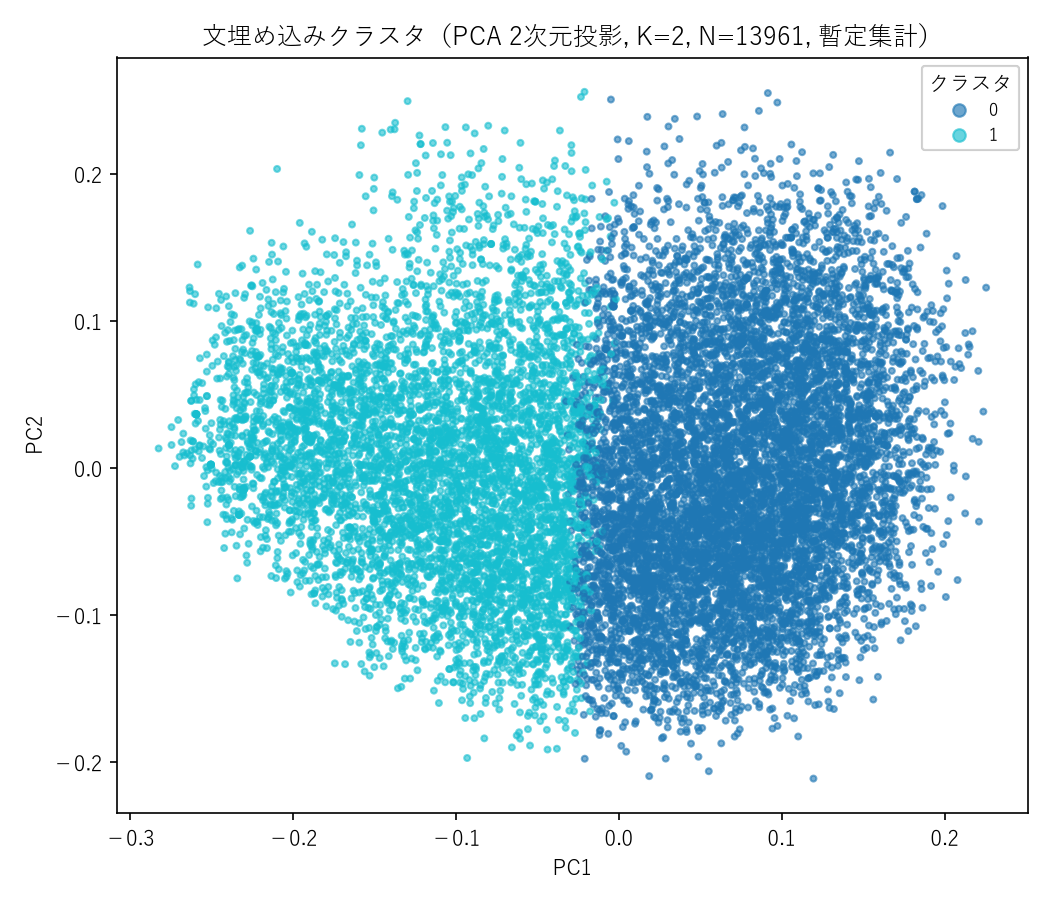
\includegraphics[width=0.75\textwidth]{coding_cluster_14501.png}
    \caption{文埋め込みによる$K$-meansクラスタリング（PCA投影，$K=2$，$N=13{,}961$）}
    \label{fig:cluster}
\end{figure}

\subsection{事前規定基準の適用}
卒論本文（\texttt{sections/04\_empirical.tex}）で結果を見る前に定めた
3基準を適用する。(i) \texttt{people\_vs\_elite}は14.56\%で1割を上回るが
\texttt{economic\_resentment}は1.98\%であり，論理和（OR）条件により
\emph{この基準は満たされる}。(ii) \texttt{blame\_target}の分布は
$p<0.000001$の高い有意差を示し，\emph{この基準は満たされない}。
(iii) \texttt{theft\_of\_enjoyment}は財務省デモ（0.8\%）・参政党
（0.8\%）ではほとんど観察されず，\emph{この基準は満たされる}。
41\%時点の判定と84\%時点の判定は完全に一致しており，「Ricci理論・
Mudde \& Rovira Kaltwasserの枠組みは，本稿が収集したYouTubeコメントの
範囲では，日本のデジタル空間における動員構造を十分に説明しない」という
事前規定の結論を採用する。

\section{コーダー内信頼性（人手検証）}
3トピックから層化抽出した57件について，著者自身がLLMの判定を見ないまま
独立に6変数を判定し，一致率とCohenの$\kappa$を算出した（二値変数の
算出は，LLMが\texttt{null}と判定した15件を除く42件を対象）。この検証は
固定サンプルに基づくものであり，コーディング件数の拡大によって変化しない。
結果は表\ref{tab:kappa}の通りである。

\begin{table}[H]
\centering
\caption{コーダー内信頼性}
\label{tab:kappa}
\begin{tabular}{lccc}
\toprule
変数 & 単純一致率 & $\kappa$ & 備考 \\
\midrule
\texttt{people\_vs\_elite} & 92.9\% (39/42) & 0.632 & 実質的な一致 \\
\texttt{economic\_resentment} & 92.9\% (39/42) & $-0.033$ & 一致は偶然水準以下 \\
\texttt{theft\_of\_enjoyment} & 92.9\% (39/42) & 0.000 & 一致なし \\
\texttt{blame\_target}（7値） & 60.5\% (26/43) & 0.468 & 中程度の一致 \\
\bottomrule
\end{tabular}
\end{table}

\textbf{重大な留保}：単純一致率はいずれも92.9\%と高いが，
\texttt{economic\_resentment}と\texttt{theft\_of\_enjoyment}の$\kappa$は
ほぼゼロである。これは両変数の出現率が数\%ときわめて低く，偶然一致率
$p_e$がすでに90\%を超える水準にあるため（「$\kappa$のパラドックス」），
わずかな不一致でも$\kappa$が大きく押し下げられることが一因だが，統計的な
不安定性だけでは説明しきれないコーディングスキームの境界事例に関する
実質的な論点も含まれている。したがって，本レポートが報告する
\texttt{economic\_resentment}・\texttt{theft\_of\_enjoyment}の出現率に
基づく結論は，測定の信頼性が実証されていない変数に基づく\emph{暫定的な
知見}として扱う必要がある。他方，\texttt{people\_vs\_elite}
（$\kappa=0.632$）は相対的に頑健な測定に基づいている。

\section{欠測パターンについての補足}
3変数（\texttt{people\_vs\_elite}等）は約15.4\%（2{,}227/14{,}501件）が
\texttt{null}であり，トピック別では参政党18.0\%，財務省デモ14.4\%，
不法移民13.9\%であった。このうち75.9\%（2{,}227件中1{,}691件）が
\texttt{emotional\_tone}の\texttt{neutral\_factual}に分類されており，
これは3変数とも判定できたコメントにおける同比率（36.6\%）の2倍以上に
あたる。この非ランダムな欠測パターンの大きさは，41\%時点（74.3\%対
35.8\%）と84\%時点（75.9\%対36.6\%）でほぼ同じであり，サンプルサイズの
拡大によって解消されない構造的な傾向であることがうかがえる。すなわち，
LLMが判断を保留しやすいコメントは，構造的に感情的な色彩が薄く，境界的・
曖昧な内容に偏っており，complete-case analysisによる出現率推定には
方向が不明な偏りが残っている可能性がある。

\section{現時点での限界}
\begin{itemize}
  \item \textbf{打ち切り時点の暫定性}：本レポートの集計は目標18{,}000件
    中84\%（$N=14{,}501$）時点のものであり，全件データに基づく結果では
    ない。ただし第\ref{sec:cutoff}節の通り，31\%・41\%・84\%の3時点を
    通じて結論は安定している。
  \item \textbf{測定信頼性}：上記の通り，\texttt{economic\_resentment}・
    \texttt{theft\_of\_enjoyment}の$\kappa$がほぼゼロであり，これらに
    基づく結論は暫定的である。
  \item \textbf{収集順序バイアス}：\texttt{order="relevance"}による収集
    のため，サンプルはエンゲージメント上位に偏っており，感情的・対立的な
    言説の出現率を過大に見積もっている可能性が高い。
  \item \textbf{分析単位の限定性}：本レポートの結果はコメント単位の
    集計であり，「日本にポピュリズムは存在するか」論争（Fahey, Hino \&
    Pekkanen対Hellmann）が要求するような，特定の政治的アクター単位の
    マクロな判定には直接接続しない。
  \item \textbf{欠測パターン}：上記の通り，欠測は完全にランダムでは
    なく，出現率の推定値には方向が不明な偏りが残る可能性がある。
\end{itemize}

\section{卒論本文との対応}
本レポートの数値はすべて，卒論本文\texttt{sections/04\_empirical.tex}
（第\ref{sec:results}節「分析2の結果と事前規定基準の適用」）に反映済み
である。\texttt{00\_abstract.tex}・\texttt{02\_japan.tex}・
\texttt{99\_conclusion.tex}中の関連数値も同時点に更新している。

\end{document}
